\label{architecture}
In this section, we present the architecture of adapting SDN-capability to
OpenNaas framework,in which we try to answer following technical questions:

\begin{figure*}[ht]
	\centering
		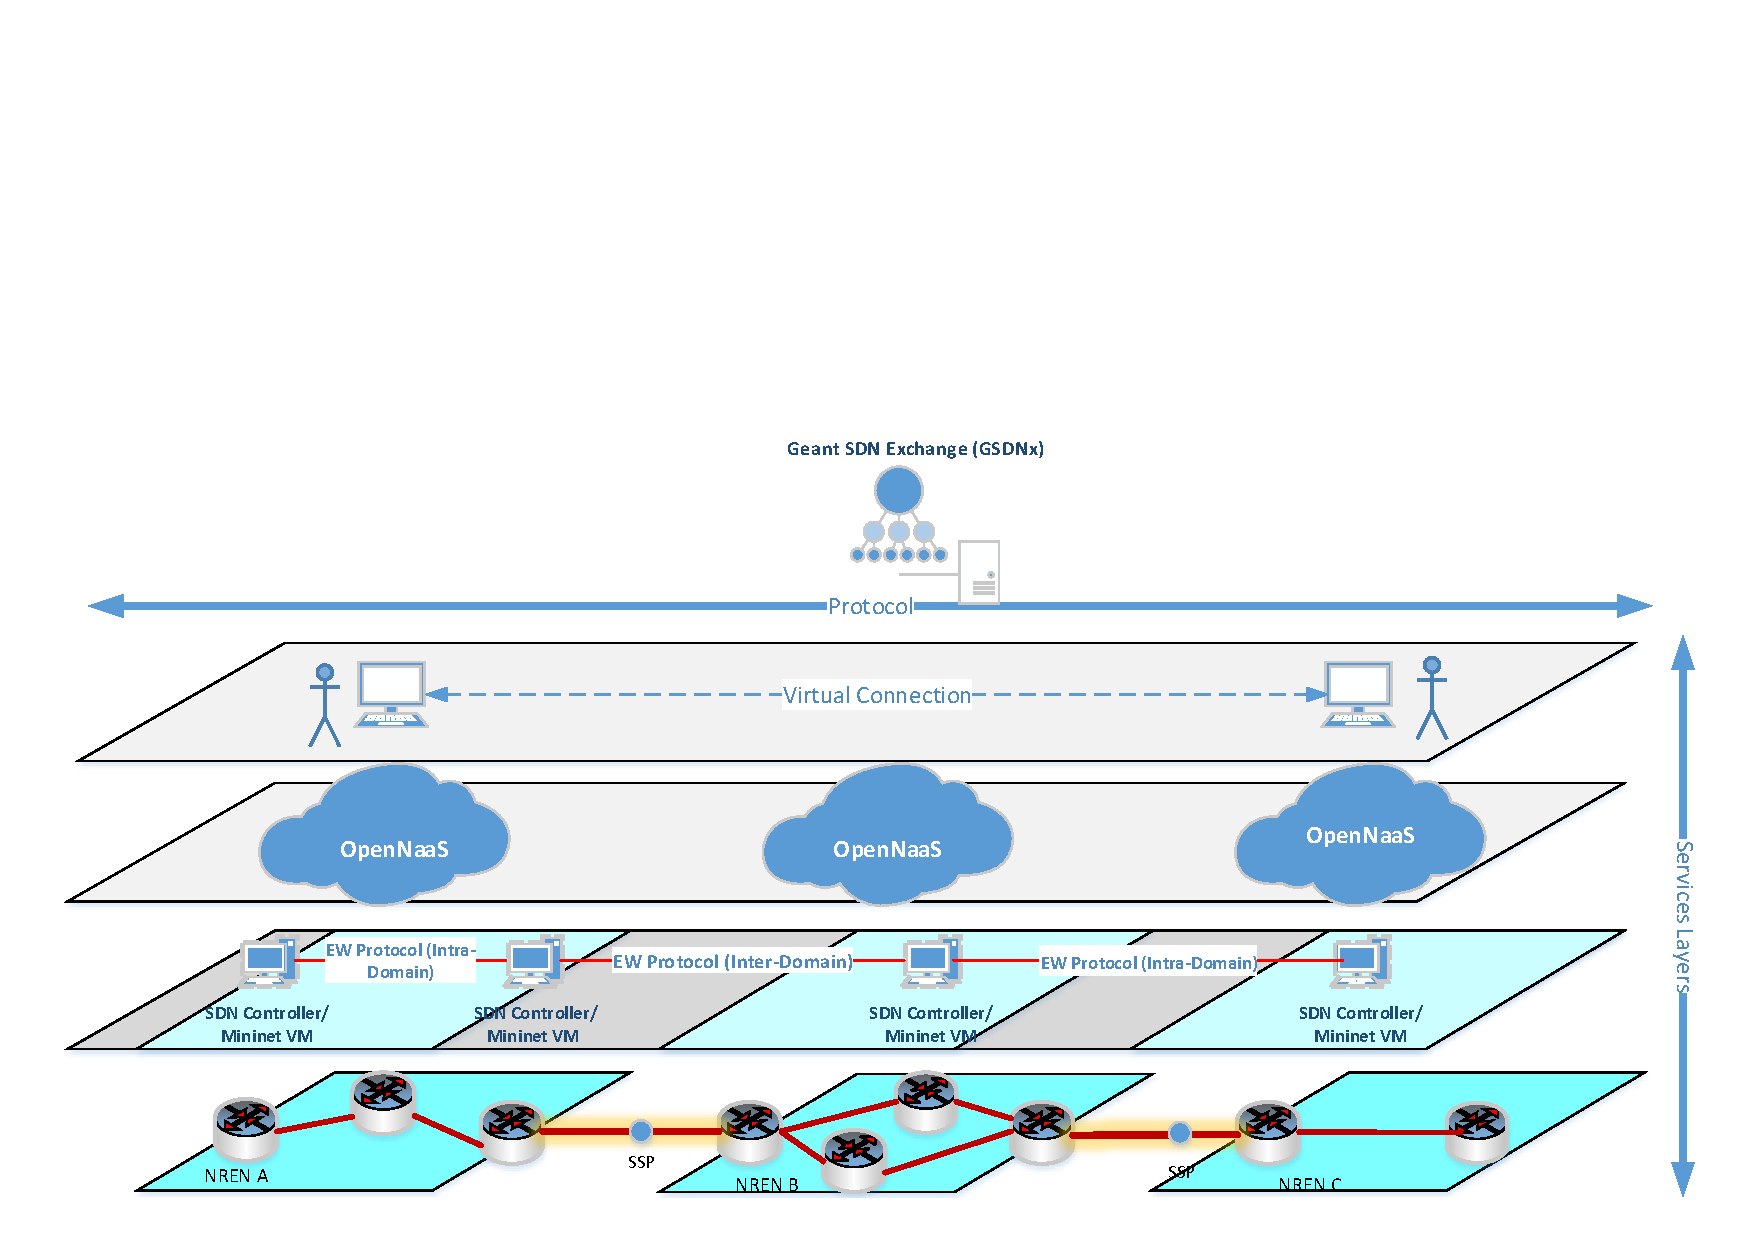
\includegraphics[width=0.7\textwidth]{GN_SDN_NaaS_Architecture.pdf}
	\caption{Architecture of Inter-domain NaaS Service over SDN Facilities}
	\label{fig:arch}
\end{figure*}

\begin{itemize}
	
	\item How to model and architect SDN-based OpenNaaS framework? 
	\item How to properly map SDN components to OpenNaaS framework?
	\item How could SDN-compatible networking devices expose their control primitives to
OpenNaaS framework and in what granularity?
	\item How to represent SDN abstractions to users and administrators of OpenNaaS framework? 

\end{itemize}

\subsection{An Architecture for Building NaaS over SDN Facility}

Figure~\ref{fig:arch} illustrates our proposal of integrating NaaS service over
SDN facilities over multiple domains. We structure the proposed architecture
into functional/service layers, where each layer provides services to its above
layers. Within layers, protocols are used to facilitate information exchanges
between different participants. Explanation regarding each layer is given as
following:

\subsubsection{Resource Layer} At bottom level of the proposed architecture,
basic data packets forwarding  capability allows simple data forwarding either
within or between domains. Note that at this layer, no routing decision is made
regarding the destinations of packets, it simply forwards data packets
according rules that are determined by the controller, thus we say the resource
layer provides data-forwarding serviced by implements rules made by the control
layer, e.g. using OpenFlow protocols. 

\subsubsection{Control Layer} The behavior of data forwarding devices at
resource layer is defined by the control layer, where standard protocol can be
used to define and communicate forwarding rules to devices forwarding table.
It is important to notice that current specifications and standards of OpenFlow
for example, do not consider East-West(EW) communications, thus collaboration
between controller is difficult, if not impossible. We argue that integration
of controller-to-controller protocols will be vital sheer from scalability
point of view. We extend OpenFlow (OF) protocols to include east-west
inter-controller communications. Since we are dealing with inter-domain
networking scenario, we need to distinguish the difference between intra- and
inter-domain controller-to-controller protocols. To the above layer, the
control layer exposes its fine granular network control interfaces in terms of,
for example, application programming interfaces (API). In term of SDN, the
controller exposes its northbound interfaces to the layer above and let it
controls the behaviour of the network more precisely and in an unified
manners.

\subsubsection{NaaS Service Layer} This layer performs actual service
provisioning process and interacts with end users of on-demand network
services. This layer determines for example  network topologies, routes and,
together with other parameters such as QoS related, NaaS service sets link
properties as end-users require and performs provisioning using services
provided by the underlying control layer. This the layer where configuration
knowledge and intelligence are located. Network parameters need to be
translated and transported on to SDN routing devices for implementation.To this
end, it is imperative that NaaS service maintain a set of well-defined
interfaces to the underlying control layer. From SDN perspective of view,
northbound interfaces in terms of loosely-coupled technologies such as RESTful
API, RPC or WebServices. Note that currently NaaS platforms such as OpenNaaS do
not support inter-domain network services, its relies on underlying layers to
provide inter-domain routing/switching capabilities by establishing virtual
networks across multiple domains.

\subsubsection{Virtual Connection Layer} This layer is responsible for actual
user perception of networking services. In Fig.\ref{fig:arch} an virtual
end-to-end (E2E) connection is illustrated, where actual packet-forwarding and
control mechanism locate in the underlying layers. Users of network service
could connect customer premises (CP) device to one of provider edge (PE) network 
devices.


\subsection{Mapping between Layers}


One of the cornerstones of the aforementioned architecture is to design a set
of well-defined interfaces for each presented layer as service primitives to
interact with their neighbouring layers. In analogie to ISO/OSI model the
functionalities of a layer are exposed by service primitives to interact with
other layers. Individual layer utlizes functions provisioned by its neighbour
abover and provides service to its under layer.

Given the fact that frameworks reside at each individual layer may have its own
interfaces makes the definitions of inter-layer interaction and mapping of
functionalities a more prominent issue to be tackled. Further more employing interfaces 
and service primitives decouples concept from its implemenetation thus renders our 
design technology-agnostic. 

\begin{figure}[htp]
	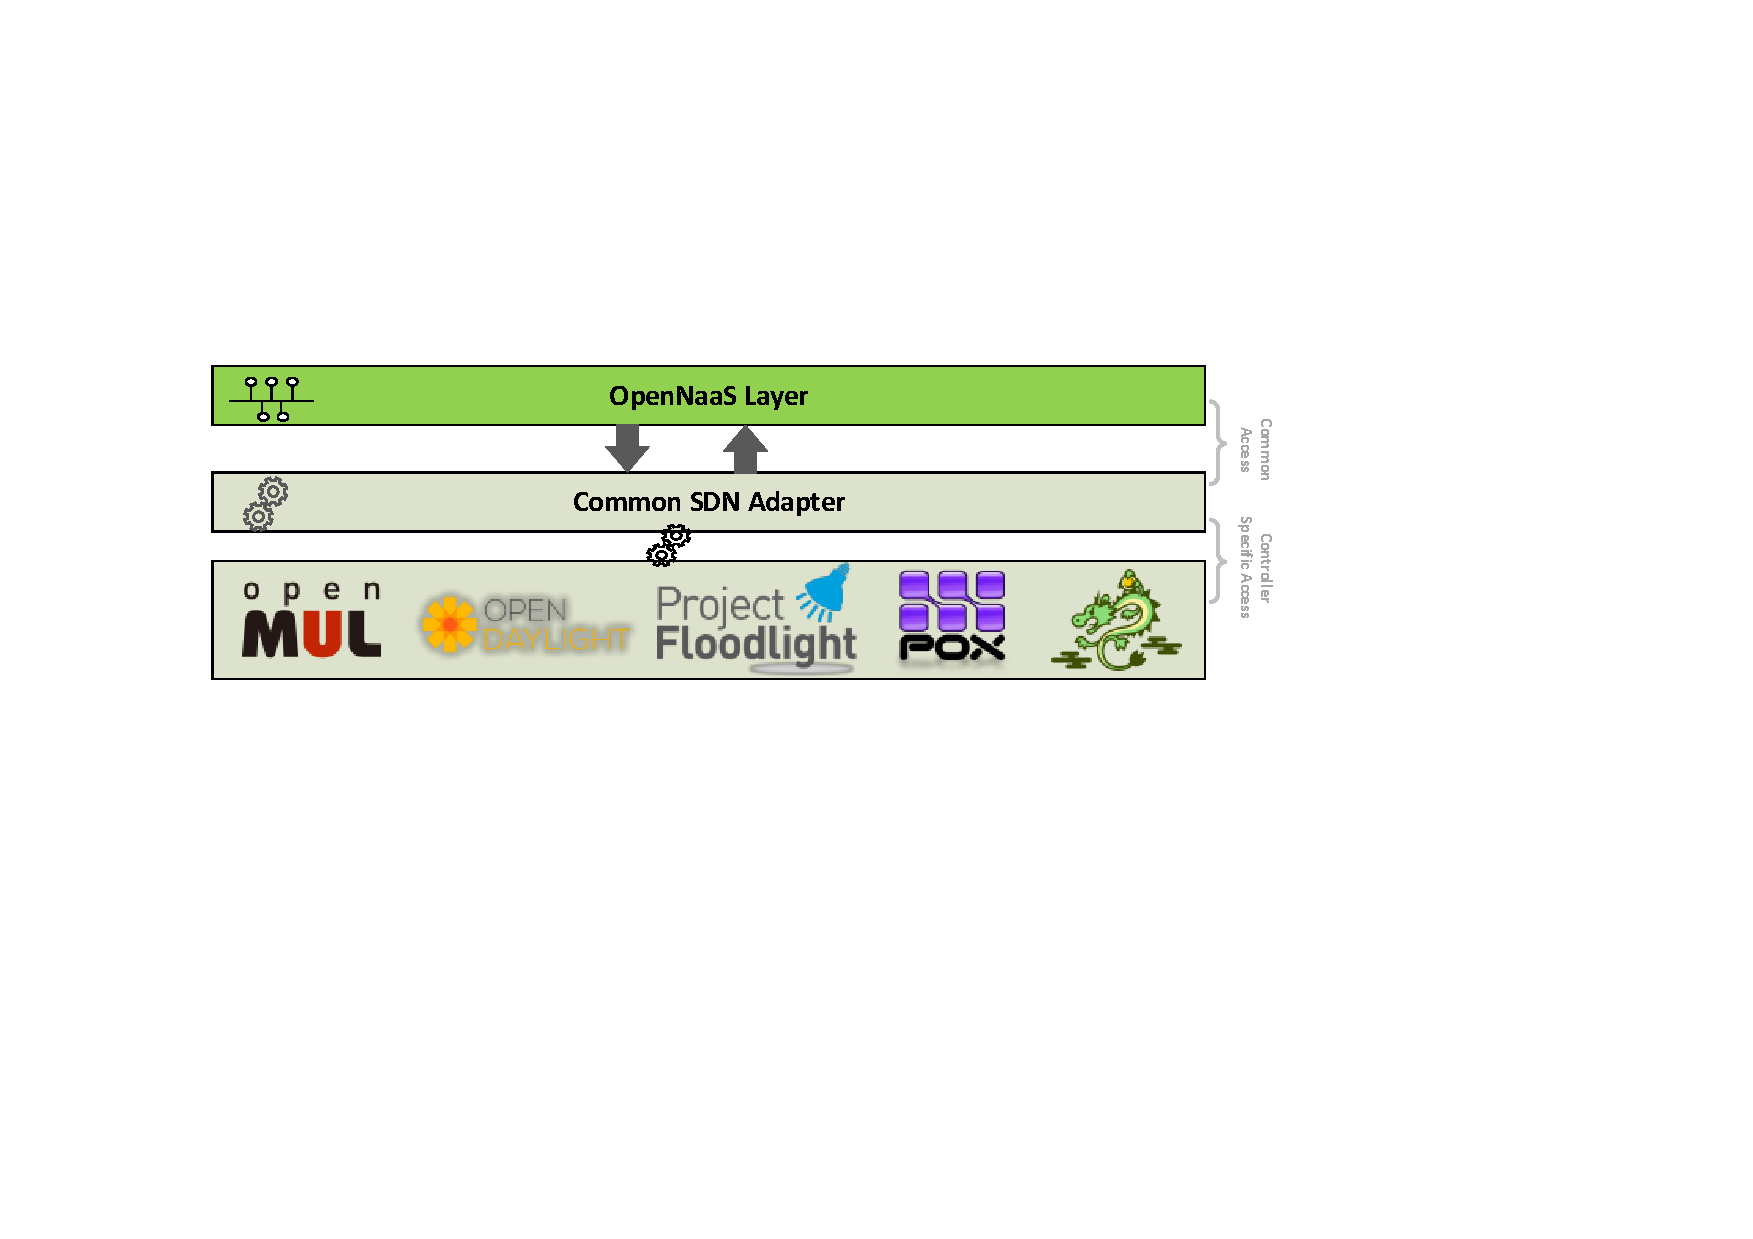
\includegraphics[scale=0.5]{controller-layer.pdf}
	\label{fig:controller-layer}
	\caption{Interactions between NaaS layer and SDN controller layer through a generic adapter}
\end{figure}


In this section, we provide detailed analysis and present our proposals for
service primitives and communication protocols between and across layers.

\subsubsection{Resource Layer Primitives \& Protocols} Service primitives of
this layer towards upper layer are defined by the OF specification from the
Open Networking Foundation (ONF). The main task for the SDN a device is
forwarding data packets in terms of flow according to flow tables and registers
network events such as incoming of data packets that do not match any
pre-defined flow rules. Contrast to conventional ones, flow tables of
SDN-capable devices can be modified at any time point by a controller. In terms
of SDN, a southbound interfaces implements OF specifications and dictates
device-to-controller communications. Note that according to specific
technologies used for the resource layer, reconfigurable protocols other than
OF can be applied as resource layer primitives~\cite{first2013}.

\subsubsection{Control Layer Primitives \& Protocols} A SDN controller exposes
its service primitives through its northbound interfaces. Unlike southbound
interfaces, definition of northbound interfaces is not standardized, it's
depends solely on the different concrete controller implementations what
services primitives in terms of API are considered. In order to make our
solution generic for all controllers, we identify a set of interfaces with
functionalities that are critical for the network management that cover
complete life-cycle of services. Provided with such information, we design an
overarching framework by applying software design
patterns~\cite{gamma1994design}. Some of potential candidates are for example
adapter, proxy and abstract factory patterns. Fig.~\ref{fig:controller-layer} illustrates 
interactions between NaaS layer and diverse controllers through a common SDN adapter.

A further issue concerning control layer protocols is the inter-domain
capability of controllers. Current specification unfortunately does not support
establishing SDN segments across multiple domains thus does not
scale~\cite{scalability2013}. Even within a domain, orchestration of multiple
controller instances are not yet well-defined. This is due the inherent
characteristics that OF based SDN is proposed and created for campus
networks~\cite{openflow08}. In order to sustain this inter-domain capability,
the current protocols have to be extended in Fig.~\ref{fig:arch} we illustrated
this extension as East-West (EW) protocol. To tackle this problem, we envision
two potential approaches:

\begin{itemize}
	\item \textit{Flow Exchanges Protocols.} To improve scalability and
		robustness of SDN based infrastructures, multiple controllers which are
		capable of exchanging informations with each others can be used to
		allow inter-controller communications and maintain a global state of
		the composed networks. To serve this goal, a EW protocol must be in
		place. Due to the differences between inter- and intra-domain
		connections, we distinguishing two types of EW protocols, respectively.

	\item \textit{Global SDN Exchange} In order to allow peering of domains in
		the global level, we propose a SDN exchange instance that allows
		exchanges of flow lables between registered SDN domains.  

\end{itemize}

\subsubsection{NaaS Service Layer Primitives \& Protocols}


\subsubsection{Virtual Connection Layer Primitives \& Protocols}
